\section{انواع فهرست‌ها}
\begin{frame}{فهرست‌ها}
\begin{itemize}\itemr
\item[-]
یکی از وابسته‌های نوشتاری بسیار مورد نیاز، تولید انواع فهرست‌هاست.

\item[-]
فهرست مطالب، فهرست عکس‌ها و فهرست جداول از فهرست‌های متداول در متون هستند.

\item[-]
نوشتن دستی فهرست‌ها از سخت‌ترین، پر غلط‌ترین و حوصله‌ سربرترین کار‌هاست.

\item[-]
به همین جهت، لاتک تگ‌هایی در اختیار ما قرار داده است که به آسان‌ترین، صحیح‌ترین و جذاب‌ترین روش این فهرست‌ها را تولید کنیم.
\end{itemize}
\end{frame}

\begin{frame}{فهرست مطالب}
\begin{itemize}\itemr
\item[-]
یکی از اصلی‌ترین فهرست‌ها، فهرست مطالب سند است.

\item[-]
برای تولید فهرست مطالب کافی‌ست که از دستور 
\lr{\texttt{\textbackslash tableofcontents}}
استفاده کرد.
\end{itemize}
\end{frame}

\begin{frame}[fragile]{نمونه کد}
\begin{latin}
\begin{lstlisting}[keywords={begin, end}, keywordstyle=\color{Mulberry}\textbf]
\begin{document}
\tableofcontents

\part{Intro}
\chapter{\LaTeX}
\section{What is \TeX}
\section{Why \LaTeX}

\chapter{Who created \LaTeX}

\part{Main}
\chapter{Structuring}
\chapter{Tables}
\section{\texttt{\textbackslash table} Environment}
\section{\texttt{\textbackslash tabular} Environment}
\section{Aligning Columns}
\end{document}
\end{lstlisting}
\end{latin}
\end{frame}

\begin{frame}{خروجی}
\begin{center}
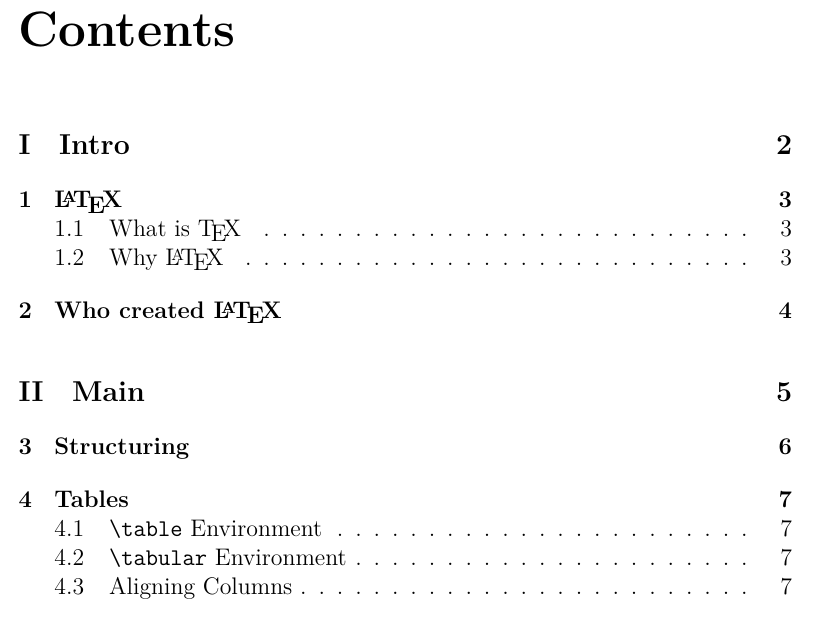
\includegraphics[width=0.7\textwidth, height=0.8\textheight]{docs/images/tab-cont}
\end{center}
\end{frame}

\begin{frame}{لینک کردن}
\begin{itemize}\itemr
\item[-]
یکی دیگر از قابلیت‌های بسیار جذاب لاتک، درست کردن لینک برای فهرست‌ها و همچنین ارجاع‌دهی‌هاست.

\item[-] 
تمام این کار توسط لاتک انجام شده و روی فایل \lr{pdf} خروجی اعمال می‌شود و تنها کار مورد نیاز ما استفاده از بسته 
\lr{\texttt{hyperref}}
است.
\end{itemize}
\end{frame}

\begin{frame}[fragile]{نمونه کد}
\begin{latin}
\begin{lstlisting}[keywords={begin, end}, keywordstyle=\color{Mulberry}\textbf]
\usepackage{hyperref}

\begin{document}
...
\end{document}
\end{lstlisting}
\end{latin}
\end{frame}

\begin{frame}{خروجی}
\begin{center}
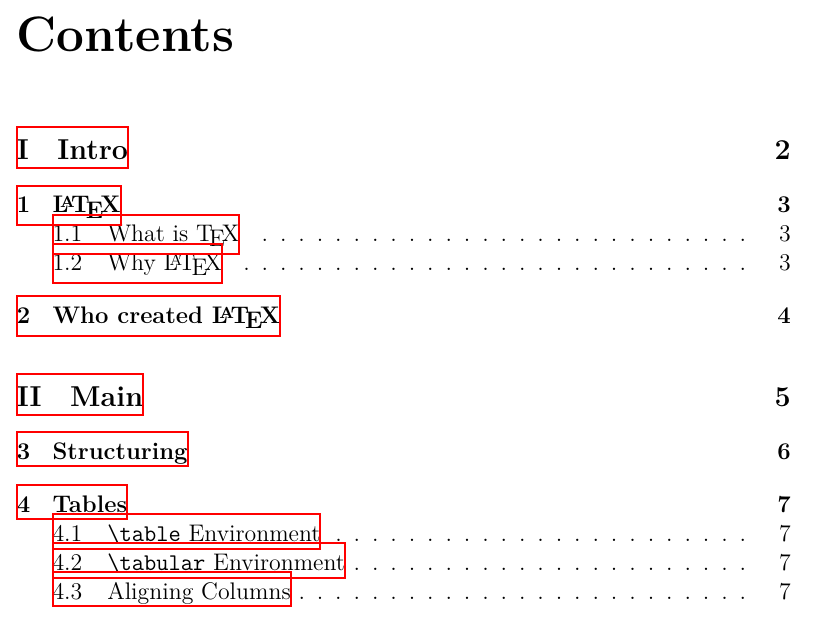
\includegraphics[width=0.7\textwidth, height=0.8\textheight]{docs/images/hyperref-simple}
\end{center}
\end{frame}

\begin{frame}{خروجی}
\begin{center}
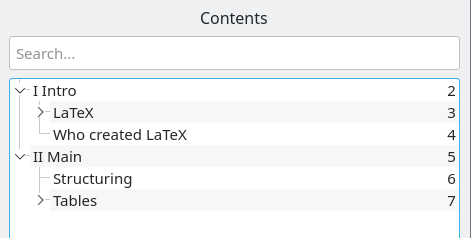
\includegraphics[width=0.5\textwidth, height=0.5\textheight]{docs/images/hyperref-affect}
\end{center}
\end{frame}

\begin{frame}{بسته \lr{\texttt{hyperref}}}
\begin{itemize}\itemr
\item[-]
مشاهده‌ کردید که تنها با استفاده از این بسته، چنین تغییراتی روی متن و فایل \lr{pdf} خروجی رخ داد.

\item[-]
اما این حالت پیش‌فرض کمی (کم نه، خیلی زیاد) زشت و ناجور است.

\item[-]
براحتی می‌توان خروجی این بسته را ویرایش کرد و به نتیجه‌ی دلخواه رسید.
\end{itemize}
\end{frame}

\begin{frame}[fragile]{نمونه کد}
\begin{latin}
\begin{lstlisting}[keywords={begin, end}, keywordstyle=\color{Mulberry}\textbf]
\usepackage{hyperref}
\hypersetup{
    colorlinks=true,
    linkcolor=blue,
    filecolor=magenta,      
    urlcolor=blue,
}

\begin{document}
...
\end{document}
\end{lstlisting}
\end{latin}
\end{frame}

\begin{frame}{خروجی}
\begin{center}
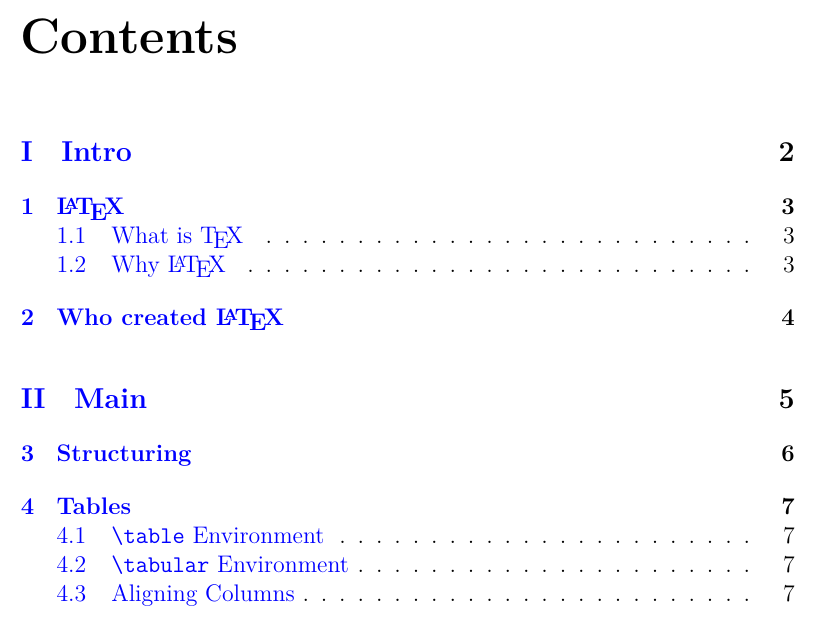
\includegraphics[width=0.7\textwidth, height=0.8\textheight]{docs/images/hyperref-edited}
\end{center}
\end{frame}


\begin{frame}{دیگر فهرست‌ها}
\begin{itemize}\itemr
\item[-]
برای تولید فهرست عکس‌ها، باید توجه داشته باشید که عکس‌ها را باید در محیط 
\lr{\texttt{figure}}
گذاشت و سپس از دستور 
\lr{\texttt{\textbackslash listoffigures}}
استفاده کرد.

\item[-]
برای تولید فهرست جداول نیز از دستور 
\lr{\texttt{\textbackslash listoftables}}
استفاده می‌شود.
\end{itemize}
\end{frame}
